\section{Practical MPC}
Practical Issues \textbf{Tracking}, \textbf{Disturbance rejection} and \textbf{Feasible Set}
\subsection{MPC for Reference Tracking}
\subsubsection{Steady-State target Problem}
reference $r$ is achieved by target state $x_S$ if $Z_s = Hx_s = r$, where $x_s$ should be a steady-state s.th. $\exists$ an input to keep system at target $x_s = Ax_s + Bu_s$\\
\fbox{\parbox{0.98\linewidth}
{\begin{minipage}{0.4\linewidth}
\begin{align*}
    x_s &= A x_s+ Bu_s \\
    Hx_S &= r 
\end{align*} 
\end{minipage}
$\Leftrightarrow$ 
\begin{minipage}{0.4\linewidth}$\begin{bmatrix}
I-A & -B \\ H & 0
\end{bmatrix} \begin{bmatrix}
x_S \\ u_S
\end{bmatrix} =  
\begin{bmatrix}
    0\\ r 
\end{bmatrix}$
\end{minipage}}}
\begin{itemize}
    \item In case of multiple feasible $u_s$, compute cheapest steady-state $(x_s,u_s)$ corresponding to $r: \mathbf{min \hspace{1mm} u_s^TR_su_s}$ subj. to \textbf{Target condition}, $x_s\in \mathcal{X},u_s \in \mathcal{U}$
    \item if $\nexists$ solution, compute reachable set point closest to $r$: 
    $\mathbf{min(Hx_s-r)^TQ_s(Hx_s-r)}$ subj to $x_s=Ax_s+Bu_s, x_S \in \mathcal{X}, u_S \in \mathcal{U}$
\end{itemize}
\vfill\null\columnbreak
\subsubsection{Delta-Formulation for Tracking}
\textbf{idea:} treat set point tracking as regulation problem with a coordinate transformation
\begin{itemize}
    \item Define deviation variables that (in the linear case) satisfy the same model equations:
    \begin{gather*}
        \Delta x = x-x_s\\ 
        \Delta u =u-u_s\\
        \Downarrow\\
        \Delta x_{k+1} = k_{k+1} -x_s \\
        = Ax_k + Bu_k - (Ax_s+Bu_s)\\
        = A \Delta x_k+ B \Delta u_k
    \end{gather*}
    \item Constraints for deviation variables: 
    \begin{gather*}
        G_xx\leq h_x \Rightarrow G_x\Delta x \leq h_x - G_x x_s \\
        G_uu\leq h_u \Rightarrow G_u \Delta u \leq h_u - G_u u_s 
    \end{gather*}
    basically subtract left and right $G_x x_s $ and $G_u u_s$
    \item Obtain target steady-state corresponding to reference $r$. 
    \item initial state $\Delta x(k) = x(k) - x_s$
    \item Apply regulation to Delta-Formulation
\end{itemize}
    \[\mathrm{min} \sum^{N-1}_{i=0} \Delta x_i^T Q \Delta x_i + \Delta u_i^TR \Delta u_i^T R \Delta u_i + V_f (\Delta x_N)\]
\begin{minipage}{0.49\linewidth}
\begin{gather*}
    \mathrm{s.t.} \Delta x_0 = \Delta x(k)\\
    \Delta x_{i+1}= A \Delta x(k)\\
    G_x\Delta x_i \leq h_x -G_xx_s \\ 
    G_u \Delta u_i \leq h_u -G_u u_s \\
    \Delta x_M \in \mathcal{X}_f
\end{gather*}
\end{minipage}
\begin{minipage}{0.5\linewidth}
    \begin{center}
        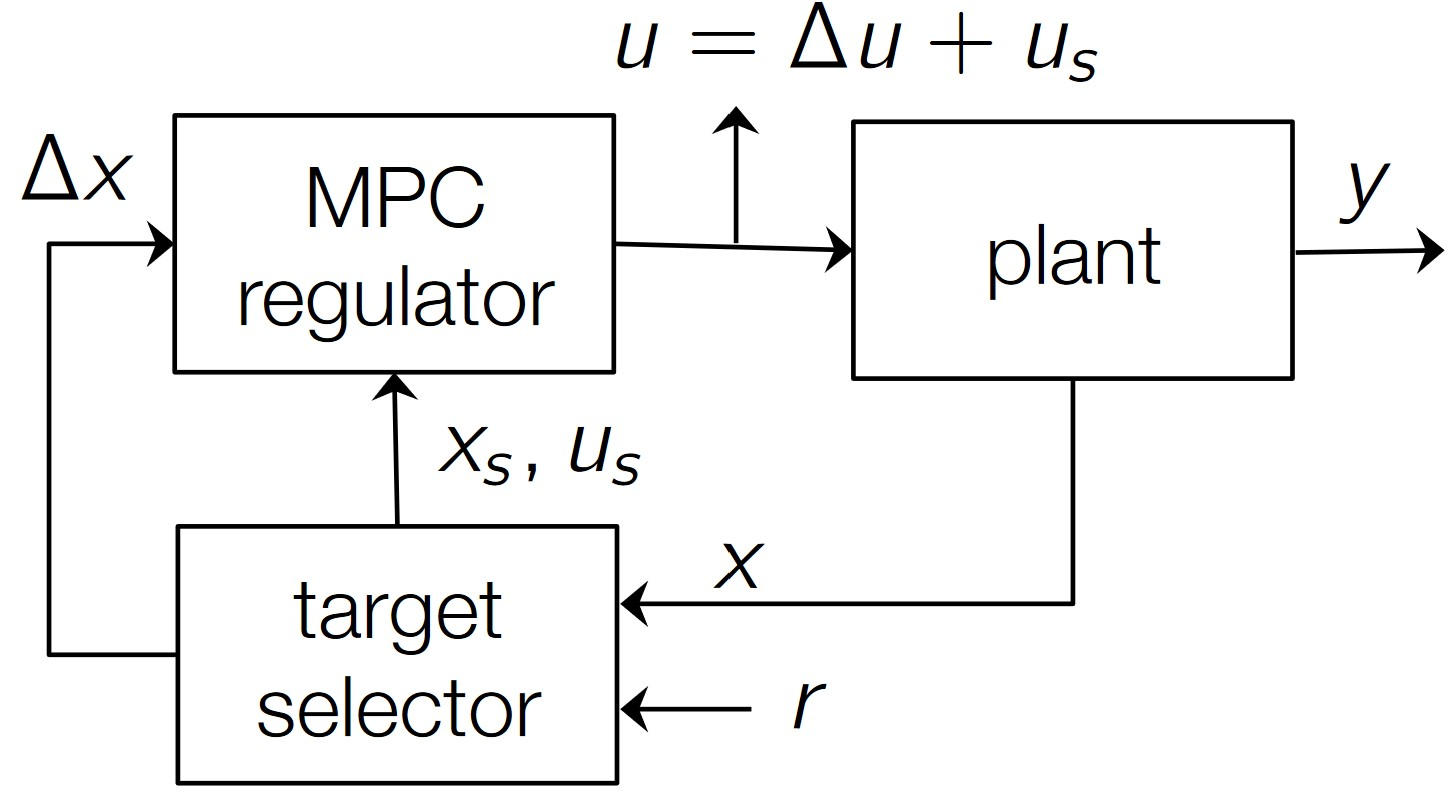
\includegraphics[width = 0.99\linewidth]{MPC_summary/Images/Screenshot 2021-07-31 220518.jpg}
    \end{center}
\end{minipage}
\textbf{Goal:} Find optimal sequence of $\Delta U^*$, input applied to the system is $u_0^* = \Delta u_0^*+u_s$
\subsubsection{Convergence}
assume target is feasible with $x_s\in \mathcal{X}, u_s \in \mathcal{U}$ and choose terminal weight $V_f(x)$ and constraint $\mathcal{X}_f$ as in the regulation case satisfying:
\begin{itemize}
    \item $\mathcal{X}_f \subseteq \mathcal{X}, Kx \in \mathcal{U} \forall x \in \mathcal{X}_f$
    \item $V_f(x(k+1)) - V_d(x(k)) \leq -I(x(k),Kx(k)) \forall x \in \mathcal{X}_f$
\end{itemize}
if in additiona the target refernce $x_s, u_S$ is s.t 
\begin{itemize}
    \item $x_s \bigoplus \mathcal{X}_f \subseteq \mathcal{X} \rightarrow x \in \mathcal{X} \forall \Delta x = x -x_s \in \mathcal{X_f}$
    \item $K \Delta x + u_S \in \mathcal{U} \forall \Delta x \in \mathcal{X}_f \rightarrow u \in \mathcal{U}$
\end{itemize}
\subsubsection{Terminal Set}
\begin{itemize}
    \item Set of feasible targets may be significantly reduced. Enlarge set of feasible targets by scalingterminal set:$\mathbf{\mathcal{X}^{scaled}_f}=\alpha \mathcal{X}_f = \{x|G_fx\leq \alpha h_f\}$
    \item If $\mathcal{X}_f$ is invariant, then $\alpha\mathcal{X}_f$ is also. chose $\alpha$ s.th. constraints are still satisfied.
    \item For targets at the \textbf{boundary of the constraints} $\mathbf{x_N = x_s}$ which corresponds to a zero terminal set $\mathcal{X}_f = 0$ because $\Delta x = x-x_S, x_N=x_s \Rightarrow \Delta x = 0.$
    $\Rightarrow$ if cl-loop system stable, set point achieved. Stability proof as for regulation.
\end{itemize}
\subsection{Constant disturbance}
Constant disturbance is acting on the system causing system trajectory to deviate from nominal dynamics
\begin{align*}
    x(k+1) &= Ax(k) + Bu(k) + B_dd\\
    y(k) &=Cx(k) + C_dd
\end{align*}
\textbf{Goal:} if system is stabilized in the presence of the disturbance then it converges to set point with zero offset.
\subsubsection{Augmented model}
\begin{align*}
    x_{k+1} &= Ax_k + B u_k + B_d d_k\\
    d_{k+1} &= d_k\\
    y_k &= Cx_k + C_dd_k\\ 
    \Downarrow \\
    A^{aug} = \begin{bmatrix} A & B_d \\ 0 & I\end{bmatrix} \hspace{2mm} C^{aug} &= \begin{bmatrix}
        C & C_d
    \end{bmatrix}
    \hspace{2mm} x^{aug} = \begin{bmatrix} x \\ d\end{bmatrix}
\end{align*}
the augmented system is \textbf{observable} iff $(A,C)$ is observable and $\begin{bmatrix} A-I & B_d \\ C & C_d \end{bmatrix}$ has full rank, i.e $\mathrm{rank} = n_x+n_d \Rightarrow$ Maximal dimension of the disturbance: $ n_d \leq  n_y$\\
Intuition: At steady-state $b\begin{bmatrix} A-I & B_d \\ C & C_d \end{bmatrix} \begin{bmatrix}x_s \\ d_s\end{bmatrix} = \begin{bmatrix}0 \\ y_s \end{bmatrix}$ and given $y_s$, $d_s$ must be uniquely defined
\vfill\null\columnbreak
\subsubsection{Linear state Estimator}
\textbf{State Observer:}
\begin{gather*}
    \begin{bmatrix}
        \hat{x}(k+1)\\
        \hat{d}(k+1)
    \end{bmatrix} =
    \begin{bmatrix}
        A & B_d \\
        0 & I
    \end{bmatrix} 
    \begin{bmatrix}
        \hat{x}(k)\\
        \hat{d}(k)
    \end{bmatrix} +
    \begin{bmatrix}
    B \\ 0
    \end{bmatrix} u(k) \\
    + \begin{bmatrix}
    L_x\\
    L_d
    \end{bmatrix}\begin{bmatrix}
    -y(k)+C(\hat{x}(k)+C_D\hat{d}(k)
    \end{bmatrix}
\end{gather*}
\textbf{Error dynamics:}\\
choose $L= \begin{bmatrix}
L_x \\ L_d
\end{bmatrix}$ such that estimator is asympt. stable
\[\begin{bmatrix}
x_{k+1}- \hat{x}_{k+1} \\
d_{k+1} - \hat{d}_{k+1} \end{bmatrix} = {\Bigg(}\begin{bmatrix}
A & B_d\\ 0 & I 
\end{bmatrix} + \begin{bmatrix}
L_x \\ L_d
\end{bmatrix} \begin{bmatrix}
C & C_d
\end{bmatrix}{\Bigg)} \begin{bmatrix}
x_k-\hat{x}_k \\ d_k- \hat{d}_k
\end{bmatrix}\]
\subsection{Enlarging the Feasible Set}
\textbf{Problem:} State/Output constraints arise from practical restrictions on the allowed operating range and are \textbf{rarely hard}. the state constraint can be \textbf{softend} by 
\begin{itemize}
    \item Minimizing the duration of the violation
    \item Minimize the size of the violation
\end{itemize}
\subsection{Soft Constrained MPC Problem Setup}
\begin{gather*}
    \underset{\mathrm{u}}{\mathrm{min}}\sum^{N-1}_{i=0}x_i^T Q x_i + u_i^T R u_i + I_\epsilon(\epsilon_i) + x_N^T P x_N+ I_\epsilon(\epsilon_N)\\
    \mathrm{s.t.} x_{i+1} = Ax_i+ Bu_i\\
    H_x x_i \leq k_x + \epsilon_i\\
    H_u u_i\leq k_u\\
    \epsilon_i\geq 0
\end{gather*}
\begin{itemize}
    \item Relax state cosntraints by introducing so called \textbf{Slack variables} $\epsilon_i \in \mathbb{R}^p$
    \item penalize amount of constrain violation in the cost by the means of penalty $I_\epsilon(\epsilon_i)$
\end{itemize}
\subsubsection{Penalties|| 7m}
\begin{itemize}
    \item Quadratic:$I_\epsilon(\epsilon_i) = \epsilon_i^T S \epsilon_i$
    \item Quadratic and linear norm penalty $I_\epsilon(\epsilon_i) = \epsilon_i^TS\epsilon_i+v||\epsilon_i||_{1/\infty}$
\end{itemize}

\begin{minipage}[]{0.49\linewidth}
\textbf{Requirement on $\mathbf{I_\epsilon(\epsilon)}$}
if the original problem has a feasible solution $z^*$, then the softend problem should have the same solution $z^*$, and $\epsilon = 0$.\\
\textbf{NOTE:} $I_\epsilon(\epsilon) = s \cdot \epsilon$ does not meet this requirement for any $s > 0$ \\
\end{minipage}
\begin{minipage}[]{0.49\linewidth}
\begin{center}
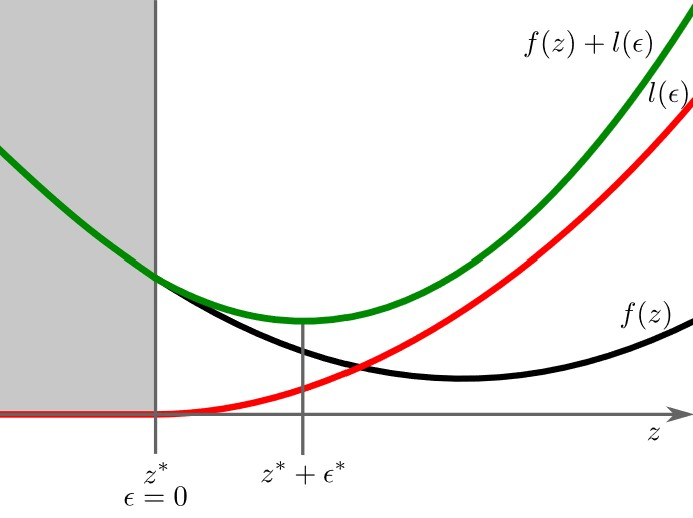
\includegraphics[width= 0.8\linewidth]{MPC_summary/Images/Quadratic_penalty.jpg}
\end{center}
\end{minipage}
\subsubsection{Tuning of Penalty Function}
\begin{itemize}
    \item \textbf{Quadratic:} Increase $S$: hardening of soft constr. $\rightarrow$ reduced size and longer duration.
    \item \textbf{Linear: }Increase $v$ results in increasing peak violation and decreasing duration.
    \begin{itemize}
        \item If weight $v$ is chosen large enough, constraints are satisfied if possible
        \item Large linear penalties make tuning difficult and cause numerical problems
    \end{itemize}
\end{itemize}
\subsubsection{Simplification: Separation of Objectives}
1. Minimize violation over horizon
\begin{gather*}
\epsilon^{\mathrm{min}}= \underset{\mathrm{u},\epsilon}{\mathrm{argmin}}\sum^{N-1}_{i=0} \epsilon^T_i S \epsilon + v^T \epsilon_i\\
\mathrm{s.t.} x_{i+1} = Ax_i + Bu_i\\
H_x x_i \leq k_x + \epsilon_i\\
H_u u_i \leq k_u\\
\epsilon_i \geq 0
\end{gather*}
2. Optimize controller performance
\begin{gather*}
    \underset{\mathrm{u}}{\mathrm{min}}\sum^{N-1}_{i=0} x_i^T Qx_i + u_i^T R u_i + x_N^T P x_N\\
    \mathrm{s.t} x_{i+1} = Ax_i + Bu_i \\
    H_x x_i \leq k_x + \epsilon^\mathrm{min}_i\\
    H_u u_i \leq k_u
\end{gather*}
$\Rightarrow$ \textbf{Advantage:} simplifies tuning, constraints will be satisfied if possible\\
$\Rightarrow$ \textbf{Disadvantage:} Requires solution of two optimization problems
